\documentclass[a4paper]{article}

\usepackage[utf8]{inputenc}
\usepackage[ngerman]{babel}
\usepackage{graphicx}
\usepackage{pdfpages}

\begin{document}
  \title{VU Objektorientierte Analyse und Design}
  \author{Gruppe 46}
  \date{9.11.2018}
  \maketitle

\section{A1}
\subsection{Klassendiagramm Hausverwaltung}

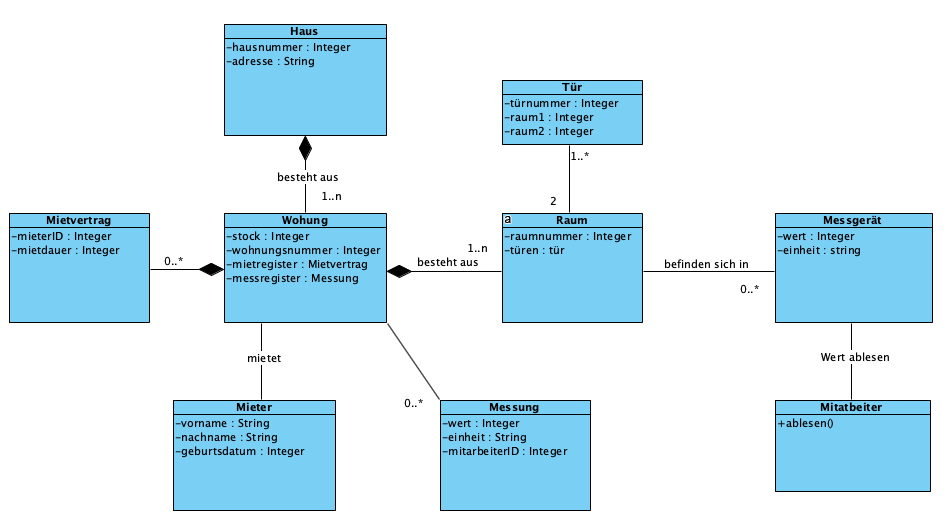
\includegraphics[width=\textwidth]{/home/zdenek/Documents/studium/sem3/OO_Analyse_Design/Project/OAD-2018-2019/Ass2/A1/Aufgabe1.png}


\section{A2}

\subsection{Business Case}

\subsubsection{Problemdefinition}

Die Anwendung T-REC soll es Usern ermöglichen, mit geringem Aufwand ein
den eigenen Interessen und Vorlieben entsprechendes Hotel zu finden. Beim
Planen seines nächsten Urlaubs ist das Angebot naturgemäß sehr groß und es
bedarf eines gewissen Aufwands, um interessante Optionen herauszufiltern. Un-
sere Produkt nimmt dem Anwender diese Arbeit ab und trifft seinen Vorlieben
entsprechend eine Vorauswahl. T-REC bringt also unsere Kunden (Hotels) ihren
Kunden (Urlaubsgäste) ein ordentliches Stück näher.

\subsubsection{Teambeschreibung und Rollen}

\begin{itemize}
\item Stefan Bortolas: Projektmanager
\item Christof Gartner: Analyst
\item Manuel Gußmagg: Usability Tester
\item Christoph Proß: Entwickler
\item Tanja Tatschl: Support
\item Zdenek Zeman: Tester
\end{itemize}

\subsubsection{Meilensteine}

\begin{itemize}
\item Organisation
\item Requirements
\item Projektstrukturplan
\item Aufgabe 1
\item GUI Prototype
\item Use Cases Diagramm
\end{itemize}

\subsubsection{Projektstrukturplan}

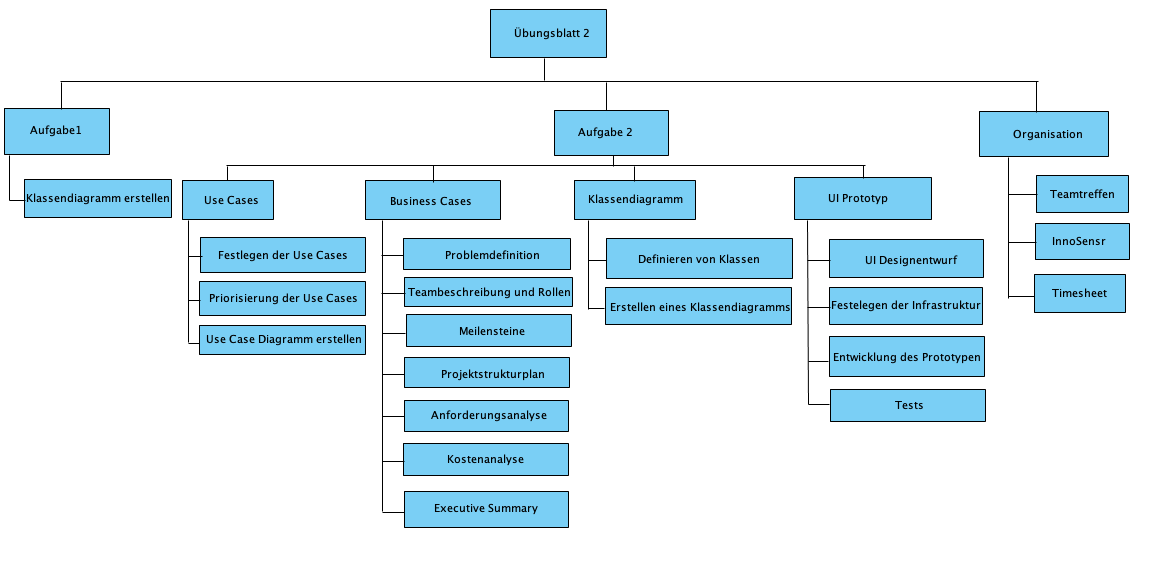
\includegraphics[width=\textwidth]{/home/zdenek/Documents/studium/sem3/OO_Analyse_Design/Project/OAD-2018-2019/Ass2/A2/Projektstrukturplan.png}

\subsubsection{Anforderungsanalyse}

Anforderungen nach Relevanz gelistet:

\begin{itemize}
\item Hotel bewerten
\item Objekte suchen
\item Aktivitäten festlegen
\item Anmelden
\item Datenbank auswerten
\item Registrieren
\item Interessensprofil verwalten
\item Statistiken anzeigen
\item Accounts verwalten
\item Empfehlungen erhalten
\item Hoteldaten verwalten
\end{itemize}

\subsubsection{Executive Summary}

Dieses Dokument wurde erstellt, um unserem Kunden die strukturierte Vorge-
hensweise in der Inseption-Phase des Projekts zu erläutern.

\subsection{Use Cases}



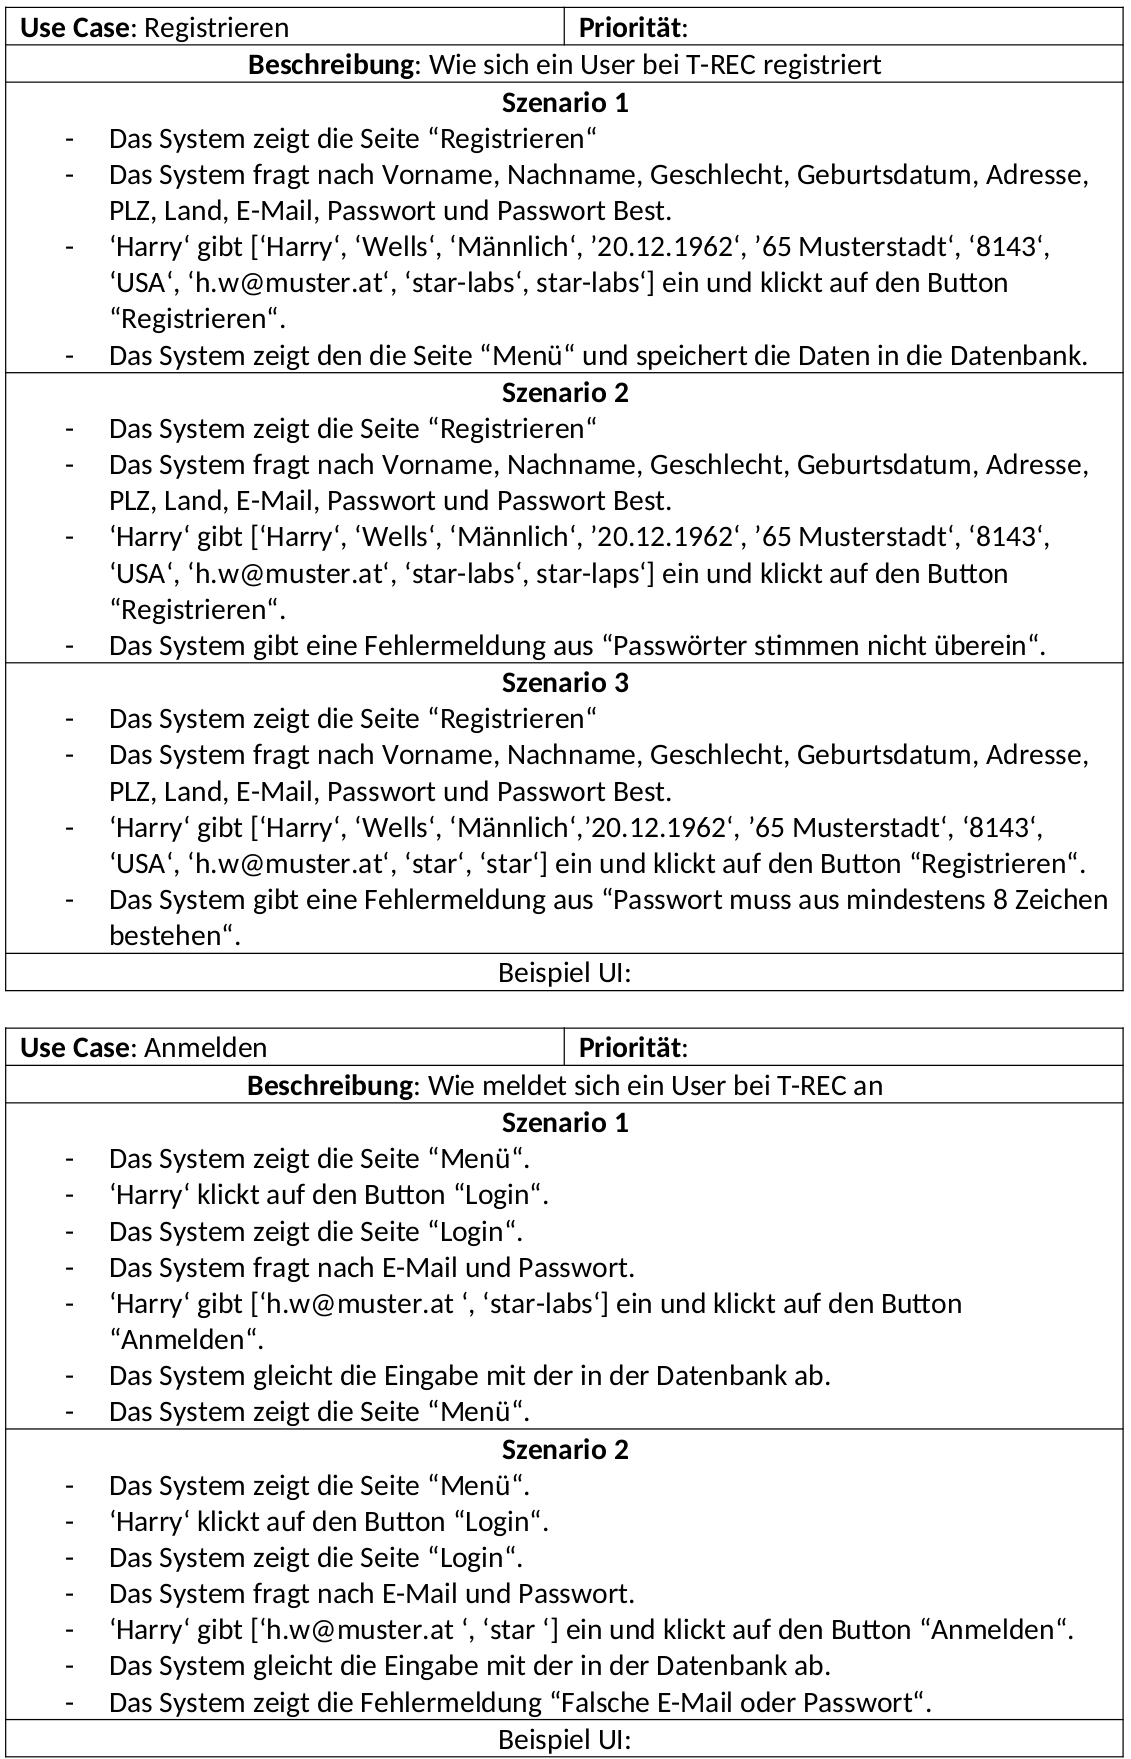
\includegraphics[width=\textwidth]{/home/zdenek/Documents/studium/sem3/OO_Analyse_Design/Project/OAD-2018-2019/Ass2/temp/use_cases_descr0.jpg}
\newpage
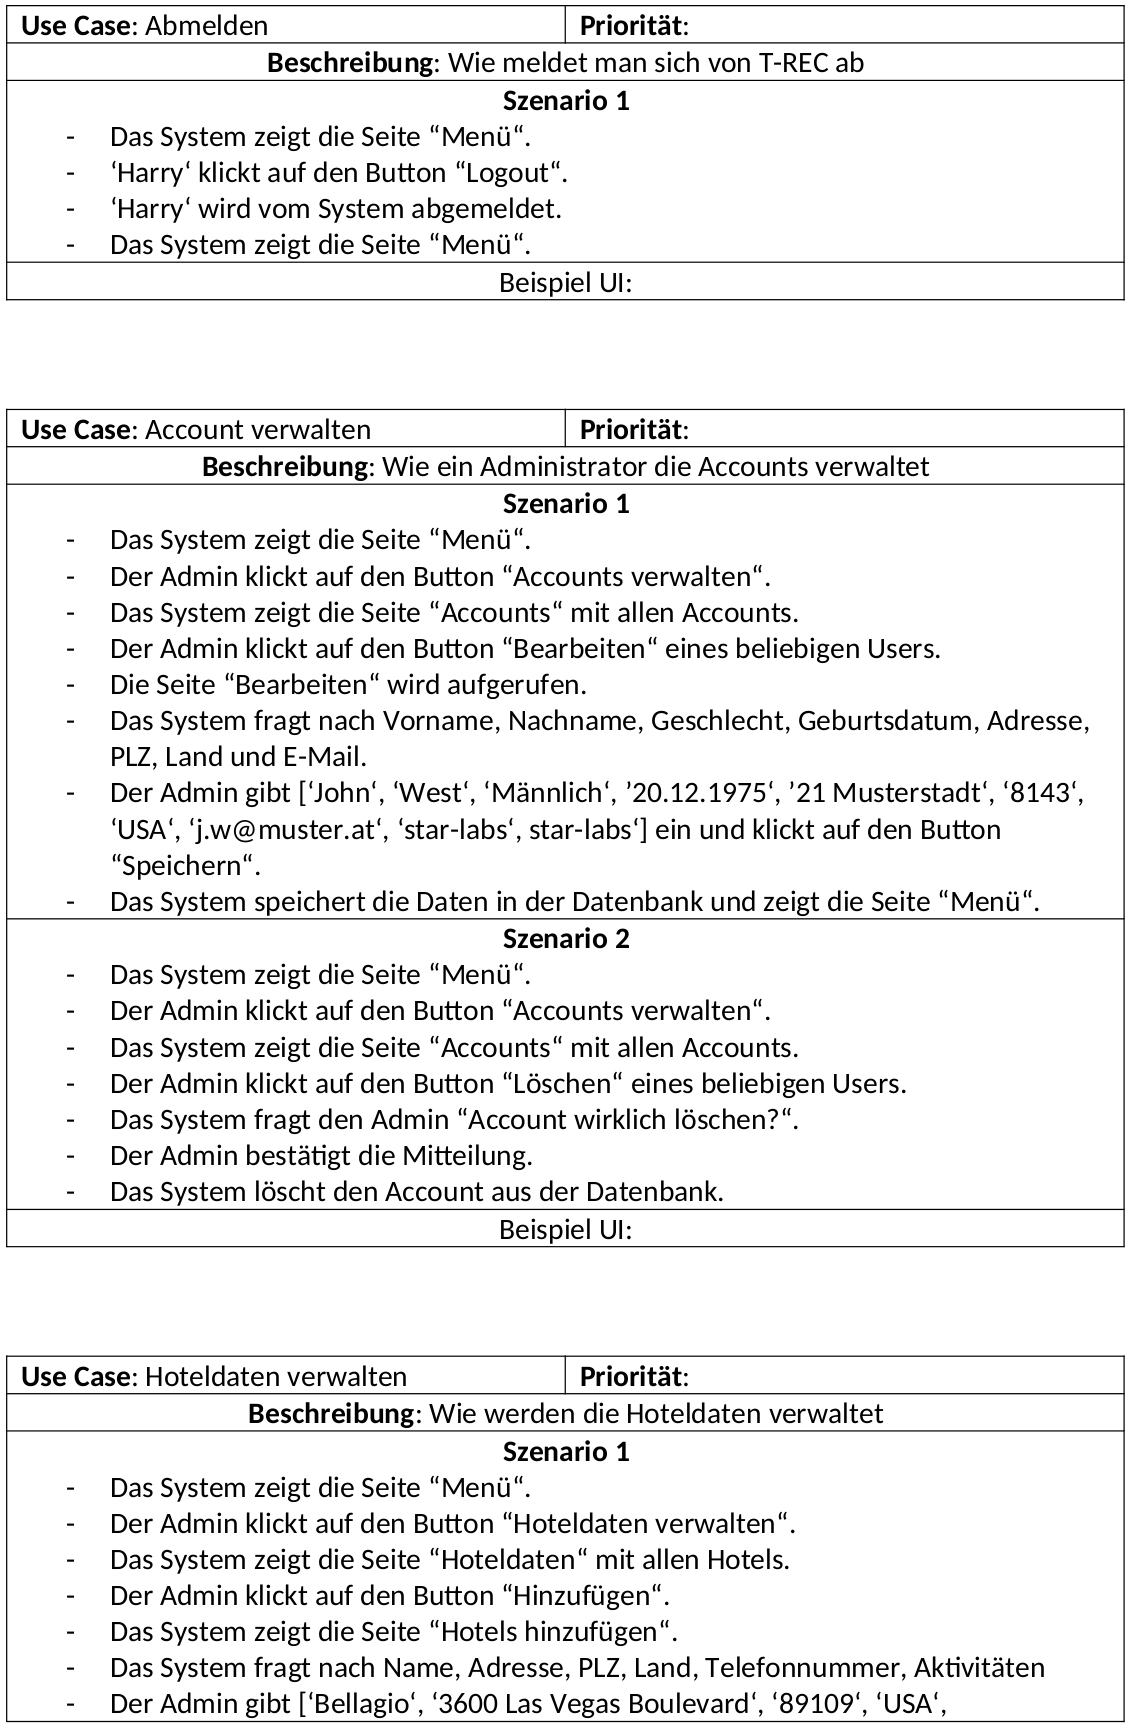
\includegraphics[width=\textwidth]{/home/zdenek/Documents/studium/sem3/OO_Analyse_Design/Project/OAD-2018-2019/Ass2/temp/use_cases_descr1.jpg}
\newpage
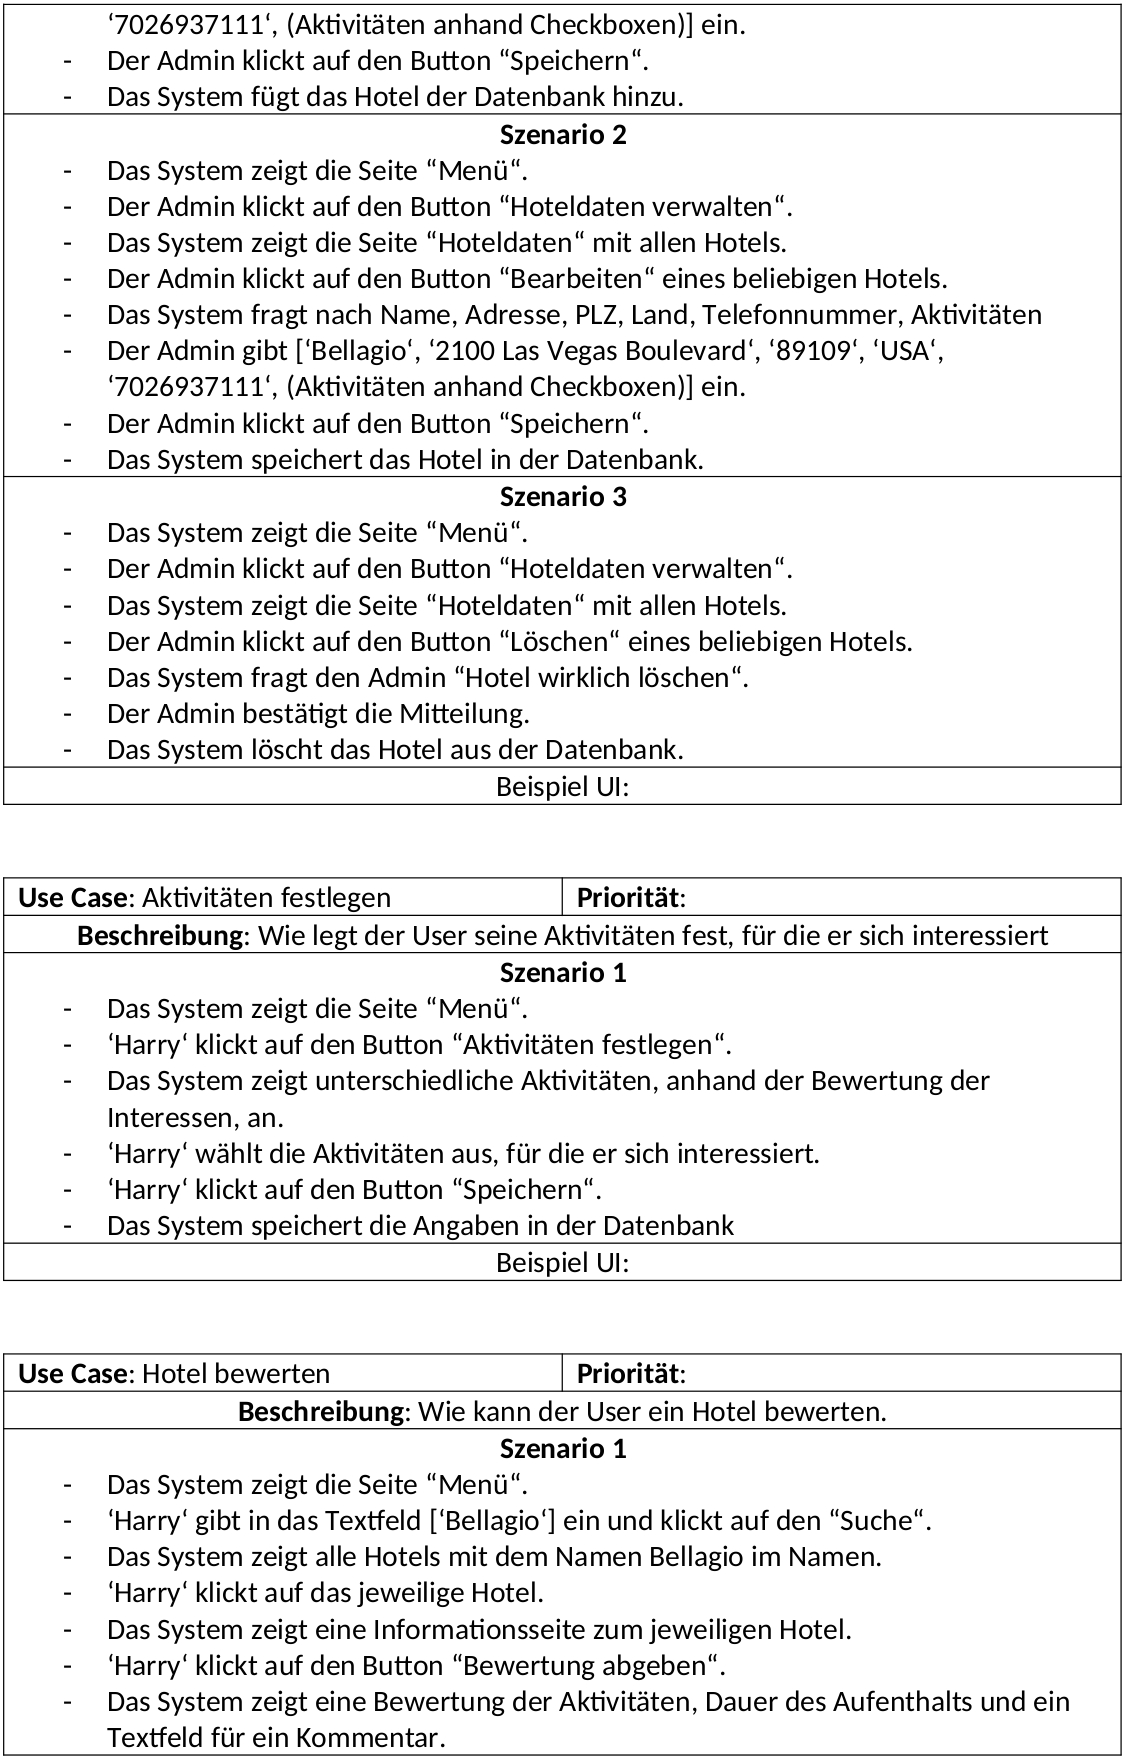
\includegraphics[width=\textwidth]{/home/zdenek/Documents/studium/sem3/OO_Analyse_Design/Project/OAD-2018-2019/Ass2/temp/use_cases_descr2.jpg}
\newpage
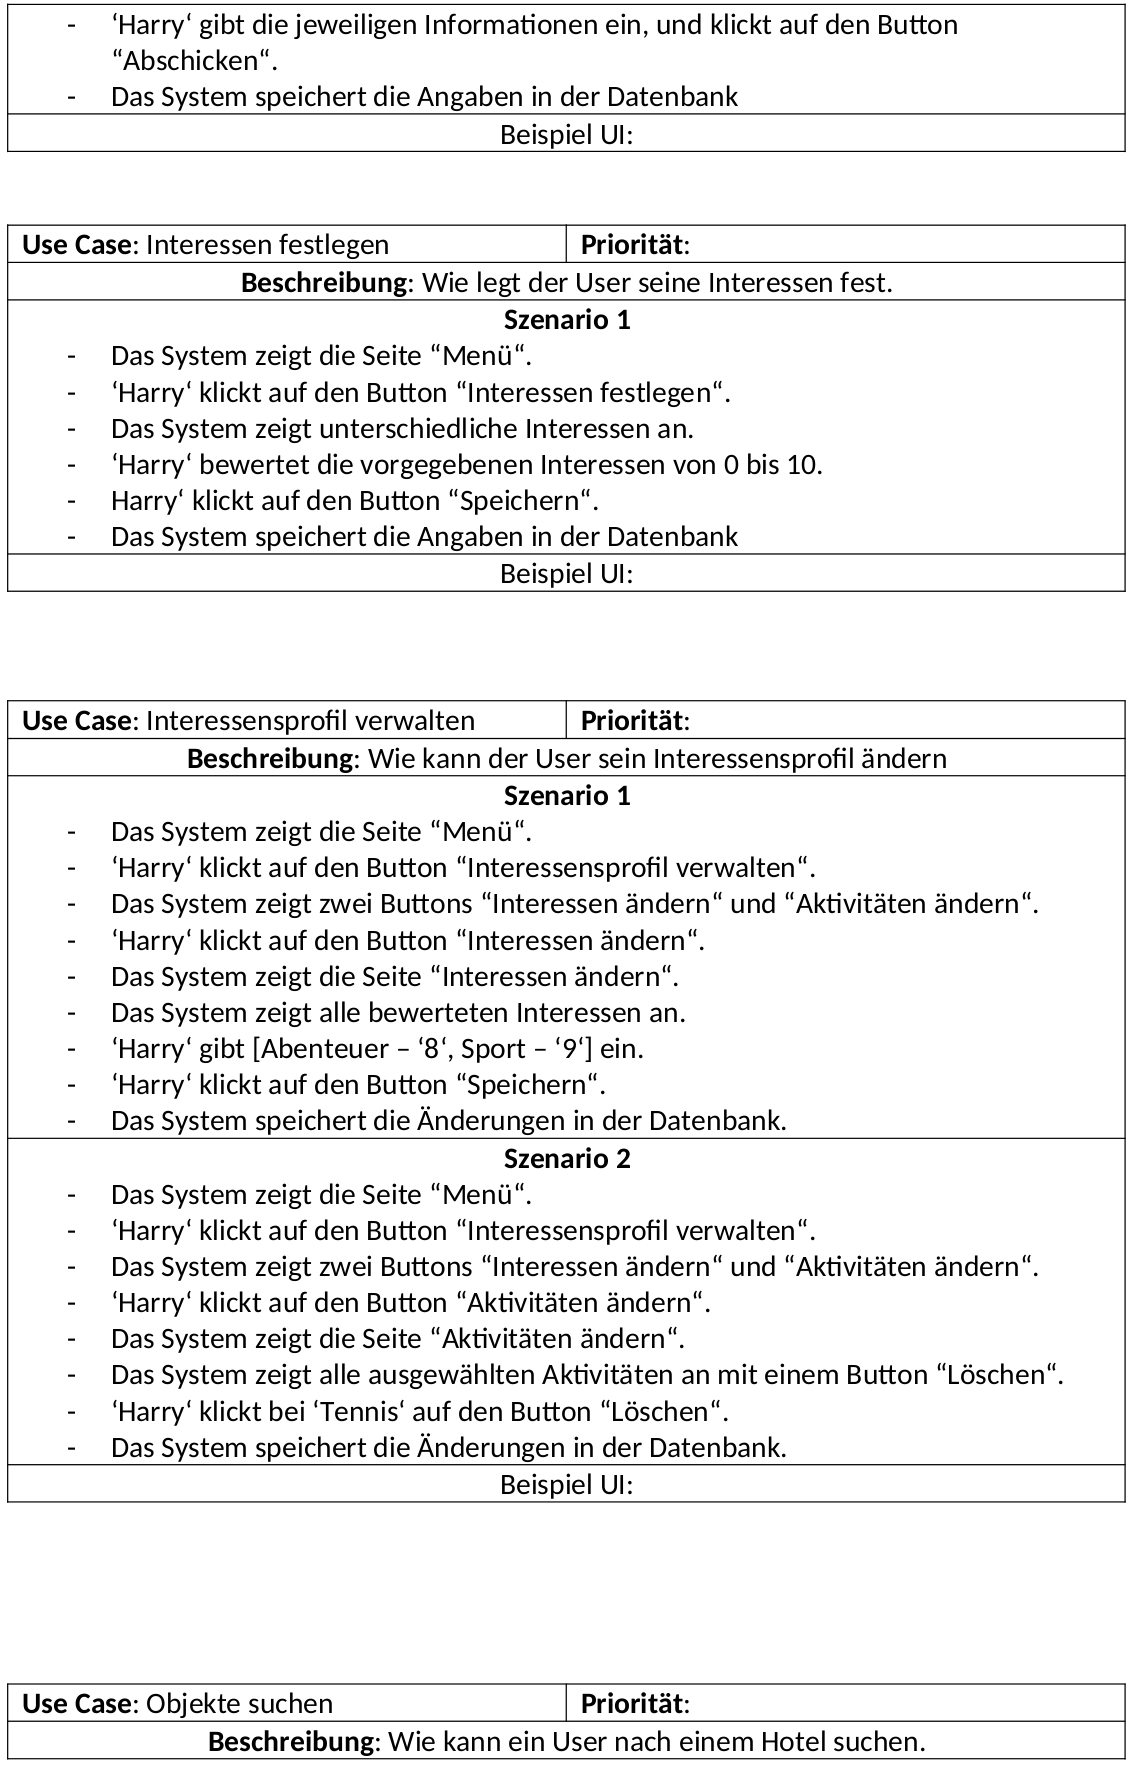
\includegraphics[width=\textwidth]{/home/zdenek/Documents/studium/sem3/OO_Analyse_Design/Project/OAD-2018-2019/Ass2/temp/use_cases_descr3.jpg}
\newpage
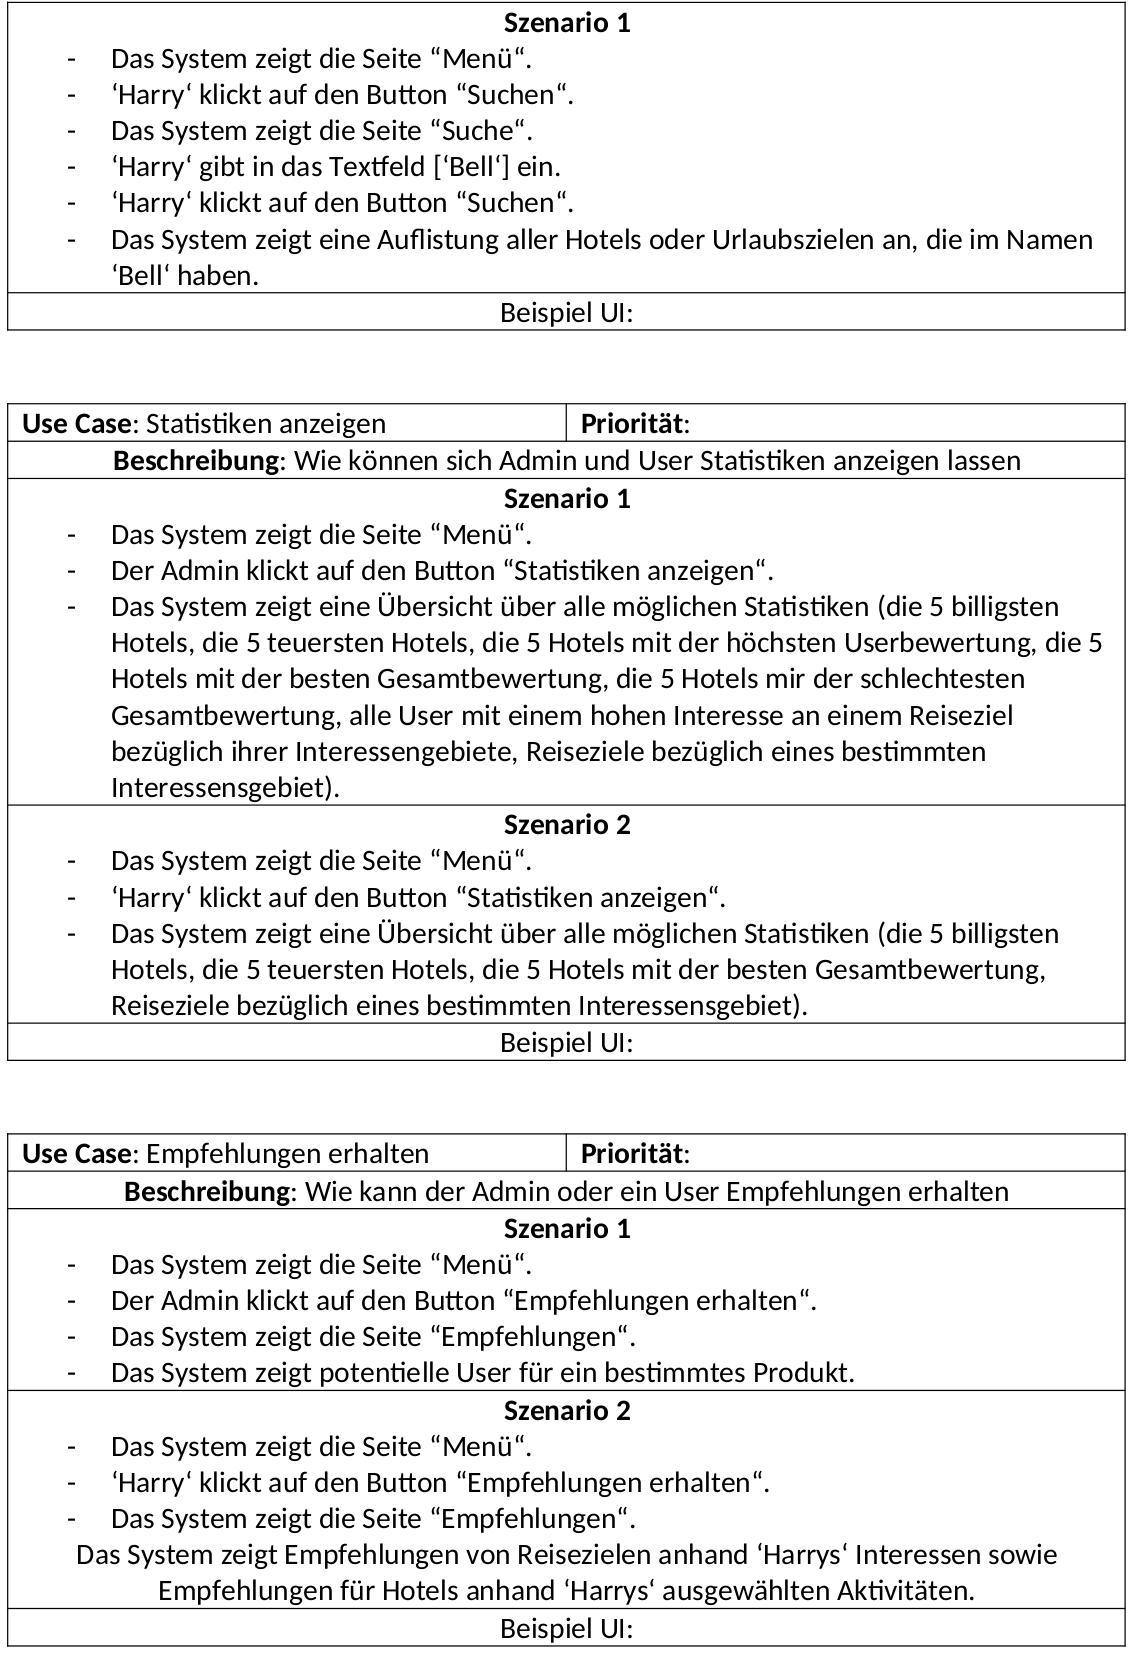
\includegraphics[width=\textwidth]{/home/zdenek/Documents/studium/sem3/OO_Analyse_Design/Project/OAD-2018-2019/Ass2/temp/use_cases_descr4.jpg}
\newpage
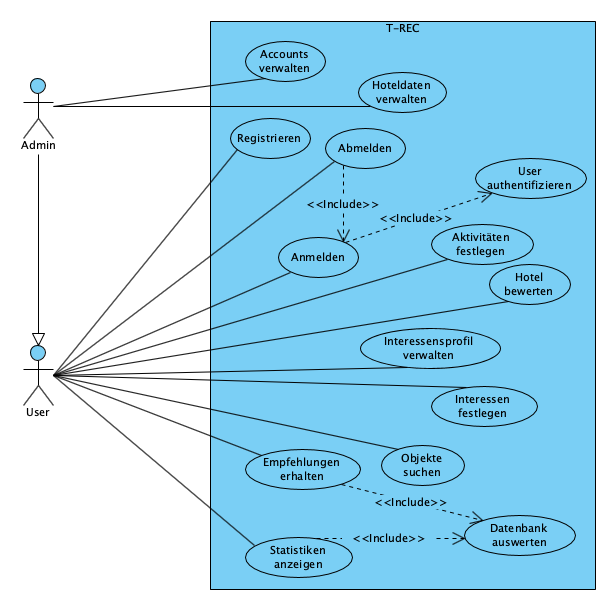
\includegraphics[width=\textwidth]{/home/zdenek/Documents/studium/sem3/OO_Analyse_Design/Project/OAD-2018-2019/Ass2/A2/Use-Case-Bild.png}

\newpage

\subsection{GUI}

Screenshots des ersten Prototypen des Graphical User Interface

\begin{figure}[h]
\centering
\caption{Anmeldung}
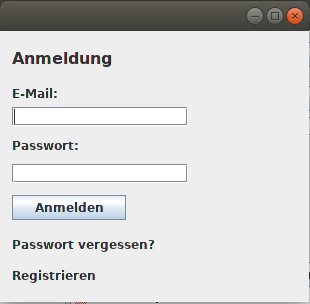
\includegraphics[width=0.5\textwidth]{/home/zdenek/Documents/studium/sem3/OO_Analyse_Design/Project/OAD-2018-2019/Ass2/A2/Ui-Screenshots/Selection_007.png}
\end{figure}

\begin{figure}[h]
\centering
\caption{Registrierung}
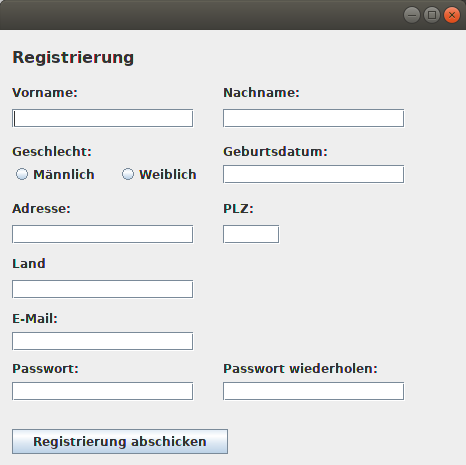
\includegraphics[width=0.5\textwidth]{/home/zdenek/Documents/studium/sem3/OO_Analyse_Design/Project/OAD-2018-2019/Ass2/A2/Ui-Screenshots/Selection_008.png}
\end{figure}

\begin{figure}[h]
\centering
\caption{Suche}
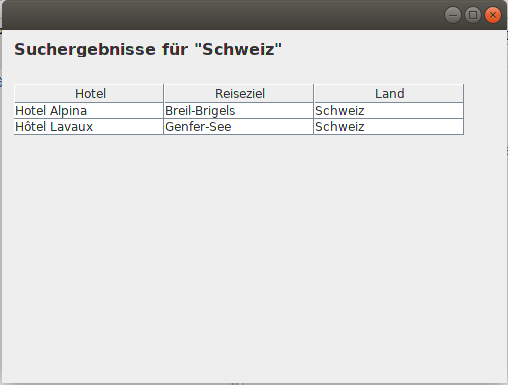
\includegraphics[width=0.5\textwidth]{/home/zdenek/Documents/studium/sem3/OO_Analyse_Design/Project/OAD-2018-2019/Ass2/A2/Ui-Screenshots/Selection_009.png}
\end{figure}

\begin{figure}[h]
\centering
\caption{Empfehlungen}
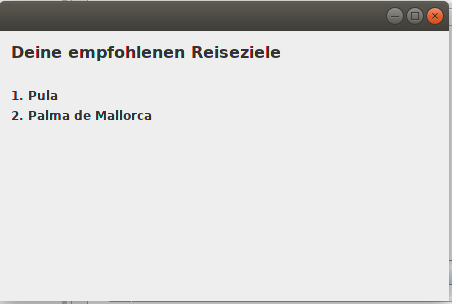
\includegraphics[width=0.5\textwidth]{/home/zdenek/Documents/studium/sem3/OO_Analyse_Design/Project/OAD-2018-2019/Ass2/A2/Ui-Screenshots/Selection_010.png}
\end{figure}

\begin{figure}[h]
\centering
\caption{Statistiken}
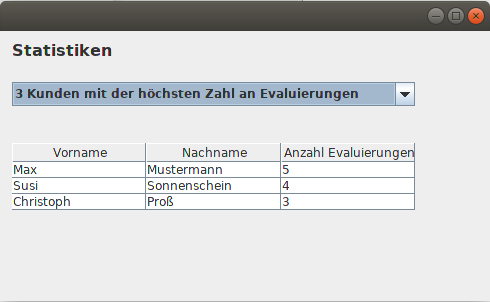
\includegraphics[width=0.5\textwidth]{/home/zdenek/Documents/studium/sem3/OO_Analyse_Design/Project/OAD-2018-2019/Ass2/A2/Ui-Screenshots/Selection_011.png}
\end{figure}

\begin{figure}[h]
\centering
\caption{Aktivitäten}
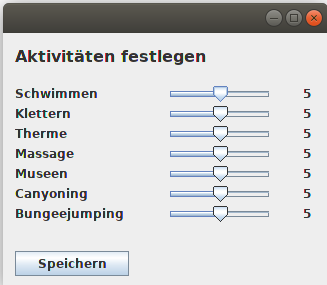
\includegraphics[width=0.5\textwidth]{/home/zdenek/Documents/studium/sem3/OO_Analyse_Design/Project/OAD-2018-2019/Ass2/A2/Ui-Screenshots/Selection_012.png}
\end{figure}

\begin{figure}[h]
\centering
\caption{Interessen}
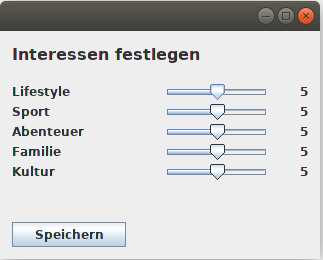
\includegraphics[width=0.5\textwidth]{/home/zdenek/Documents/studium/sem3/OO_Analyse_Design/Project/OAD-2018-2019/Ass2/A2/Ui-Screenshots/Selection_014.png}
\end{figure}

\begin{figure}[h]
\centering
\caption{Hoteldetails}
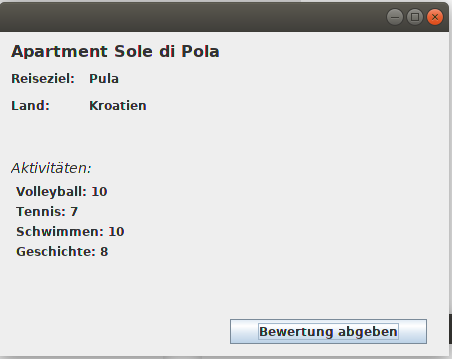
\includegraphics[width=0.5\textwidth]{/home/zdenek/Documents/studium/sem3/OO_Analyse_Design/Project/OAD-2018-2019/Ass2/A2/Ui-Screenshots/Selection_015.png}
\end{figure}

\begin{figure}[h]
\centering
\caption{Hotelbewertung}
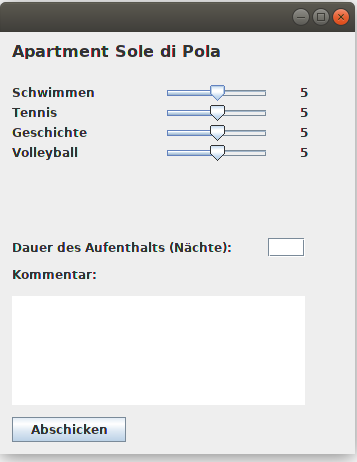
\includegraphics[width=0.5\textwidth]{/home/zdenek/Documents/studium/sem3/OO_Analyse_Design/Project/OAD-2018-2019/Ass2/A2/Ui-Screenshots/Selection_016.png}
\end{figure}

\begin{figure}[h]
\centering
\caption{Home}
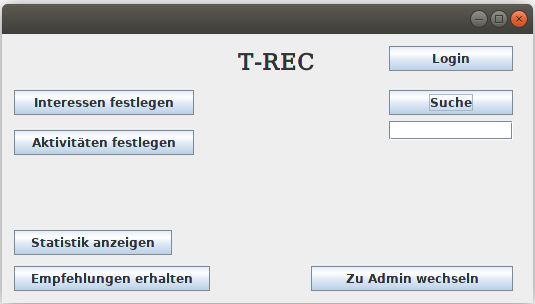
\includegraphics[width=0.5\textwidth]{/home/zdenek/Documents/studium/sem3/OO_Analyse_Design/Project/OAD-2018-2019/Ass2/A2/Ui-Screenshots/Selection_017.png}
\end{figure}


\end{document}